
現在已經有了基準測試來測量讀寫內存的速度,看看如何訪問內存中的數據,可以獲得最佳性能。先從隨機存取開始,讀或寫的每個值的位置都不可預測。

\subsubsubsection{4.4.1\hspace{0.2cm}隨機訪存的速度}

如果不多次運行基準測試,並對結果進行平均(基準庫可以做到這一點),那麼測量結果可能會相當混亂。在合理的運行時間(分鐘)內,可能會看到如下結果:

%\hspace*{\fill} \\ %插入空行
\begin{center}
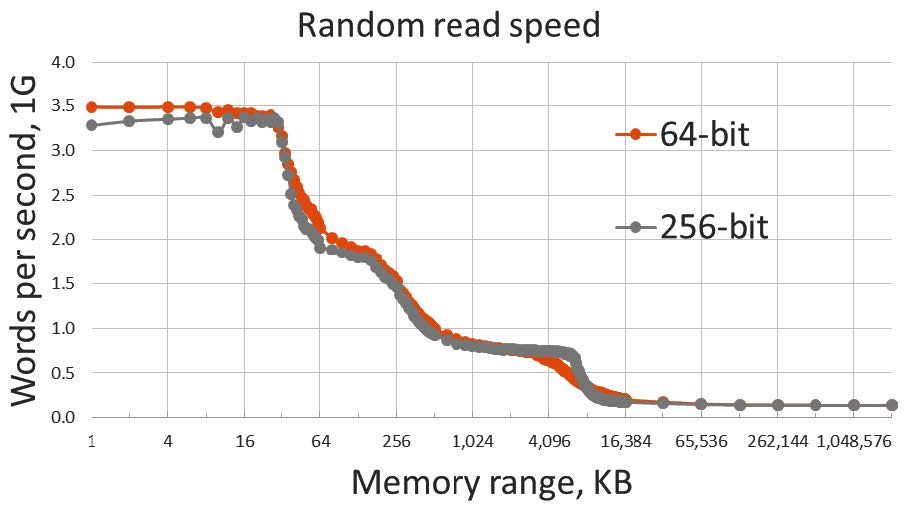
\includegraphics[width=0.9\textwidth]{content/1/chapter4/images/3.jpg}\\
圖4.3 - 隨機讀取速度與內存大小的關係
\end{center}

圖4.3中的基準測試結果顯示,每秒從內存中讀取的數據(以十億為單位),長度為64位整數或265位整數(分別為\texttt{long}或\texttt{\_\_m256i})。同樣的值也可以表示為,讀取指定大小的單個整數所花費的時間:

%\hspace*{\fill} \\ %插入空行
\begin{center}
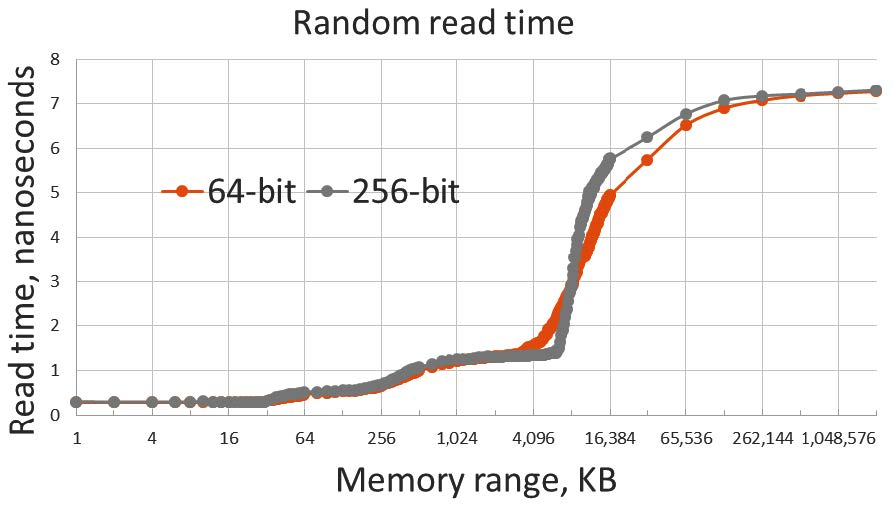
\includegraphics[width=0.9\textwidth]{content/1/chapter4/images/4.jpg}\\
圖4.4 - 讀取一個數組元素的時間與數組大小的關係
\end{center}

首先,沒有單一的內存速度。在我所使用的計算機上,讀取一個64位整數所需的時間從0.3納秒到7納秒不等。讀取少量數據要比讀取大量數據快得多。可以從這些圖中看到緩存的大小,32KB的L1緩存速度很快,數據量都能裝入L1緩存,讀取速度就不依賴於數據量。超過32KB的數據,讀取速度就開始下降。數據現在適合L2緩存,它更大(256KB),但速度更慢。數組越大,適合快速L1緩存的部分就越少,訪問速度越慢。

如果數據從L2緩存溢出,讀取時間會增加得更多,必須使用L3緩存。不過,L3緩存要大得多,所以直到數據大小超過8MB時才會發生變化。這時,才真正開始從主存讀取數據。數據都是在第一次接觸時從內存中移動到緩存中的,所有後續的讀取操作都只使用緩存。如果需要一次訪問超過8MB的數據,那麼其中的一些數據必須從主內存中讀取(不同的CPU模型的緩存大小不同)。當然,不要馬上去除緩存的好處是,只要大多數數據適合於緩存,至少在某種程度上是有效的。當數據量超出緩存大小几倍,讀取時間完全取決於從內存中檢索數據所花費的時間。

在緩存中找到某個變量進行讀或寫,稱之為\textbf{緩存命中}。如果沒有找到,就註冊一個緩存缺失事件。當然,L1緩存缺失可以是L2命中。一個L3緩存缺失意味著必須從主存加載數據。

從內存中讀取一個整數需要7納秒。按照處理器的標準,這是非常長的時間,CPU每納秒可以做幾個操作。還需要注意的是,CPU可以在從內存中讀取一個整數值所花費的時間,可以執行大約50個算術運算,除非該值恰好已經在緩存中。很少有程序需要對每個值執行50個操作,這意味著CPU很可能沒有得到充分利用,除非能夠找到一些加速內存訪問的方法。

最後,以每秒整數為單位的讀取速度並不取決於整數的大小。從實用的角度來看,如果使用256位的指令來讀取內存,可以讀取4倍的數據。當然,SSE和AVX加載指令可以將值讀入不同的寄存器,因此還可以使用SSE或AVX SIMD指令進行計算。更簡單的情況是,只需要將大量數據從內存中的一個位置複製到另一個位置。測試表明,複製256位字比64位字快4倍。當然,現在有了庫函數可以進行內存複製,比如:\texttt{memcpy()}或\texttt{std::memcpy()},並對其進行了優化,以獲得最佳的效率。

速度不依賴於數據大小這一事實還有另一個暗示,讀取速度受延遲影響,而不是帶寬的限制。延遲是發出數據請求和檢索數據之間的事件。帶寬是內存總線在給定時間內可以傳輸的數據總量。從64位到256位在同一時間內傳輸的數據是64位的4倍。也就是,我們還沒有達到帶寬限制。這似乎是一個純理論的結論,它確實對編寫高效程序有重要的影響。

最後,我們可以測試寫入內存的速度:

%\hspace*{\fill} \\ %插入空行
\begin{center}
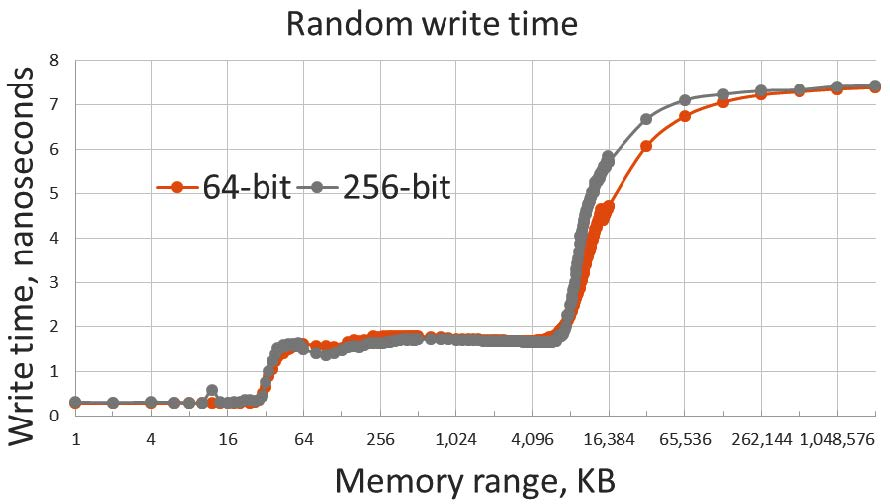
\includegraphics[width=0.9\textwidth]{content/1/chapter4/images/5.jpg}\\
圖4.5 - 數組元素的寫入時間與數組大小的關係
\end{center}

隨機讀寫有非常相似的性能,但是這會因不同的硬件而不同。在前面觀察到的讀取內存的速度也適用於寫入,在圖4.5中看到了緩存大小的影響。如果涉及到主內存,則寫入的總體等待時間會非常長,而且一次寫入多個詞會更有效率。

能否得出內存訪問對性能影響的結論?一方面,如果需要重複訪問少量的數據(小於32KB),就不必為此擔心。當然,重複是這裡的關鍵,無論計劃訪問多少內存,第一次訪問的內存位置都必須接觸主存(直到讀取整個數組並返回開始,計算機才知道數組很小——第一次讀取一個小數組的第一個元素看起來與讀取第一個元素完全一樣大數組的)。另一方面,如果必須訪問大量的數據,那麼內存速度可能會成為首先關心的問題:7納秒/個的速度,能等得起嗎?

有幾種提高內存性能的技術,將會在本章中看到。我們也會研究如何改進我們的代碼,先看看硬件。

\subsubsubsection{4.4.2\hspace{0.2cm}順序訪存的速度}

我們已經測試了在任意位置訪問內存的速度,每一次內存訪問實際上都是新的。我們正在讀取的整個數組會加載到能夠放入的最小緩存中,然後隨機讀寫該緩存中的不同位置。該數組不適合緩存,然後隨機訪問內存中的不同位置,並且每次訪問(對於我使用的硬件)都會產生7納秒的延遲。

隨機訪存在程序中經常發生,但同樣頻繁的是順序訪存,從第一個元素到最後一個元素的順序處理一個大數組。這裡的隨機和順序訪問是由存儲器地址的順序決定的,有可能出現誤解的是,鏈表是不支持隨機訪問的數據結構(意味著不能直接跳到列表的中間),必須從頭元素開始按順序訪問。如果每個鏈表元素在不同的時間分配,那麼順序遍歷列表很可能是以隨機順序訪問內存。另一方面,數組是一種隨機訪問數據結構(可以隨時訪問任何元素)。然而,從數組的開始讀取到結束,順序訪問內存,按照單調遞增的地址順序。除非另有說明,在本章討論順序訪問或隨機訪問時,只關心訪問內存地址的順序,而非數據結構。

順序訪存的性能也與隨機方式不同。下面是順序寫入的結果:

%\hspace*{\fill} \\ %插入空行
\begin{center}
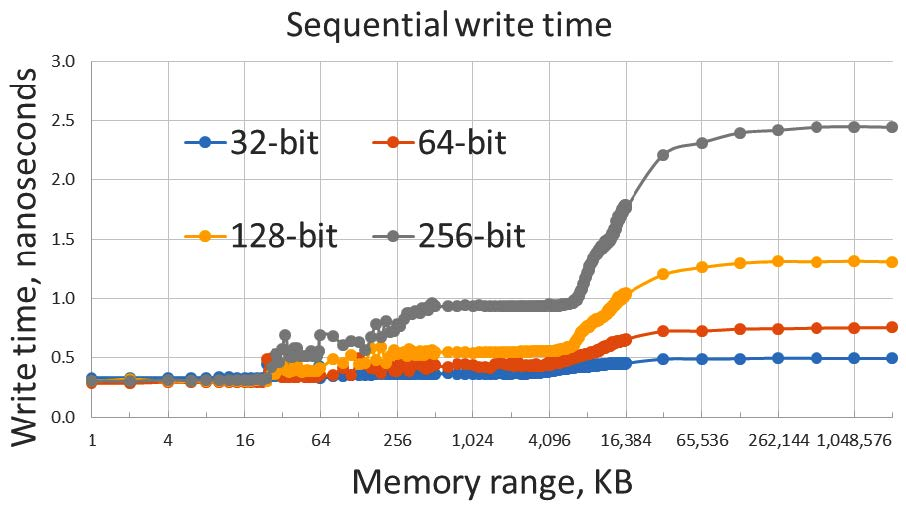
\includegraphics[width=0.8\textwidth]{content/1/chapter4/images/6.jpg}\\
圖4.6 - 順序訪存,數組元素的寫入時間與數組大小的關係
\end{center}

圖的整體形狀和以前一樣,但不同之處和相似之處同樣重要。首先,需要注意的是縱軸的刻度,時間值比我們在圖4.5中看到的要小得多。寫一個256位的值只需要2.5納秒,而64位的整數只需要0.8納秒。

第二個區別是數據塊不同時,曲線不再相同。需要注意的是,此結果高度依賴硬件。許多系統中,將會看到與前一節中的結果更加相似的結果。在我使用的硬件上,對於不同大小的數據塊,L1緩存的順序寫時間是相同的,但對於其他緩存和主存則不同。在主存寫入時,可以觀察到,寫入64位整數的時間,並不是寫入32位整數所需的時間的兩倍,對於更大的數據,每次數據量加倍時,寫入時間都加倍。這說明,限制不是每秒可以寫多少個數據塊,而是每秒可以寫多少個字節:對於所有數據塊的大小(除了最小的一個),每秒寫入的字節數是相同的。現在限制速度的不是延遲,而是帶寬。以總線能夠傳輸的最快速度推送到內存中,無論將它們分為64位的數據塊,還是256位的數據塊,現在都已經達到了內存的帶寬限制。本章中,這個結果比之前所做的觀察更加依賴硬件。在許多機器上,會出現內存足夠快,而CPU無法飽和使用其帶寬的情況。

雖然與緩存大小相對應的曲線中的“階梯”仍然可見,但不那麼明顯,也不那麼陡峭。現在已經有了結果,也進行了觀察。那結論是什麼呢?

\subsubsubsection{4.4.3\hspace{0.2cm}硬件中的內存性能優化}

三個觀察結果需要結合起來,可以看出硬件使用了某種隱藏延遲的技術(除了改變內存訪問順序外,沒有做任何事情來提高代碼的性能,所以這些改進都歸功於硬件)。當隨機訪問主內存時,每次訪問在我的機器上需要7納秒。這是從特定地址的數據請求到交付至CPU寄存器所花費的時間,這個完全由訪存延遲決定(不管請求了多少字節,必須等待7納秒)。當按順序訪問內存時,硬件可以開始傳輸數組的下一個元素。訪問第一個元素仍然需要7納秒,順序訪問內存時,硬件可以馬上訪問數組的下一個元素。第一個元素仍然需要7納秒來訪問,此後硬件以CPU和內存總線處理它的速度將整個數組從內存中寫入或讀出。數組中第二個和之後元素的傳輸,有可能在CPU發出數據請求之前就開始了。因此,延遲不再是限制因素,而帶寬才是。

當然,這是假設硬件已知要按順序訪問整個數組,以及這個數組有足夠大。在現實中,硬件什麼都不知道,就像上一章學習的條件指令一樣,內存系統中有學習迴路,可以做出有根據的猜測。在我們的示例中,出現了\textbf{預取}。當內存控制器注意到CPU已經連續訪問了幾個地址,就會假設這個地址會繼續使用,併為訪問下一個內存位置做準備,將數據傳輸到L1緩存中(用於讀操作),或者在L1緩存中騰出空間(用於寫操作)。理想情況下,預取技術允許CPU始終以L1緩存的速度訪問內存,當CPU需要每個數組元素時,其已經在L1緩存中了。實際情況是否符合這種理想情況,要取決於CPU在訪問相鄰元素之間做了多少工作。在基準測試中,CPU幾乎不做任何工作,而預取則落後了。期望線性順序訪問,則沒有辦法足夠快地在主內存和L1緩存之間傳輸數據。然而,預取在隱藏內存訪問延遲方面非常有效。

預取並不是基於如何訪問內存的預測或先驗(有一些特定於平臺的系統調用,允許程序通知硬件某個範圍的內存將被順序訪問,但這是不可移植的,而且在實踐中很少奏效)。相反,預取嘗試在訪問內存時檢測訪存模式。因此,預取的有效性取決於,訪存模式和下一次訪問的位置。

關於預取模式檢測的侷限性有很多信息,其中很多都已經過時。在較早的文獻中,可以讀到按向前順序訪問內存(對於數組\texttt{a},從\texttt{a[0]}到\texttt{a[N-1]})比向後訪問更高效。這對現代CPU來說都不再適用,而且現在已經不是這樣了。如果我開始準確地描述,哪些模式在預取方面是有效的,哪些模式是無效的,那麼該書就有落入同樣陷阱的風險。最後,如果算法需要特定的內存訪問模式,並且想知道預取能否處理它,最可靠的方法是使用與隨機內存訪問類似的基準測試進行測試。

通常,預取對於訪問內存的遞增順序和遞減順序都有效。在預取調整到新的模式之前,反轉方向會有一些性能損失。像訪問數組中的每4個元素這樣的跨步處理,會被檢測和預測,其效率與密集的順序訪問一樣。預取能夠檢測多個併發跨步(即訪問每3個和每7個元素),但當硬件功能從一個處理器轉移到另一個處理器時,必須自己對數據進行緊緻化處理。

硬件非常成功地採用的另一種性能優化技術:\textbf{流水線}或\textbf{硬件循環展開}。在上一章中我們已經瞭解過,這種技術可以用來隱藏由條件指令引起的延遲。通常,流水線也可用於隱藏內存訪問的延遲。看一下這個循環:

\begin{lstlisting}[style=styleCXX]
for (size_t i = 0; i < N; ++i) {
	b[i] = func(a[i]);
}
\end{lstlisting}

每次迭代從數組中讀取一個值\texttt{a[i]},進行一些計算,並將結果存儲在另一個數組\texttt{b[i]}中。讀和寫都需要時間,可以期望循環執行的時間軸是這樣的:

%\hspace*{\fill} \\ %插入空行
\begin{center}
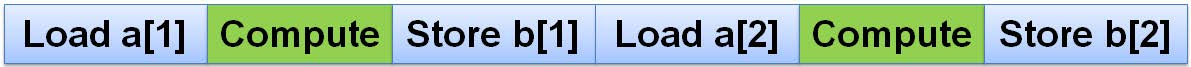
\includegraphics[width=0.9\textwidth]{content/1/chapter4/images/7.jpg}\\
圖4.7 - 非流水線循環的時間線
\end{center}

這個操作序列會讓CPU在大部分時間裡等待內存操作完成。硬件將提前讀入指令流,並覆蓋彼此不依賴的指令序列:

%\hspace*{\fill} \\ %插入空行
\begin{center}
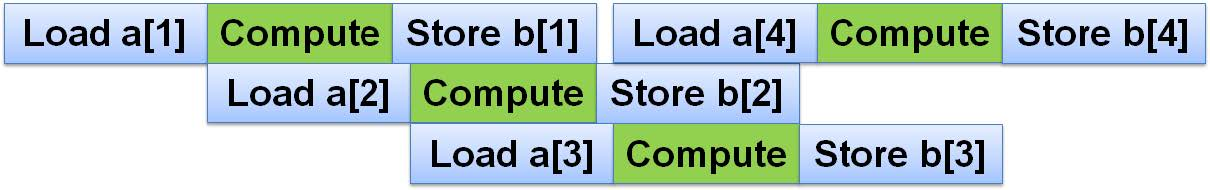
\includegraphics[width=0.9\textwidth]{content/1/chapter4/images/8.jpg}\\
圖4.8 - 流水線(展開)循環的時間線
\end{center}

假設有足夠的寄存器,第二數組元素的加載可以在第一個數組元素讀取後立即開始。簡單來說,假設CPU不能一次加載兩個值(大多數真正的CPU可以同時做多個內存訪問,這意味著流水線可以更寬),當有輸入值可用,第二組計算就開始。前幾個步驟中,指令載入流水,CPU花費了大部分時間進行計算(如果來自不同迭代的計算步驟重疊,CPU甚至可以一次執行多個迭代,只要有足夠多的計算單元)。

流水線可以隱藏內存訪問的延遲,但這是有限制的。讀取一個值需要7納秒,需要讀取一百萬個值,最多需要7毫秒,這是無法避免的(假設CPU一次只能讀取一個值)。流水線操作可以通過將計算與內存操作重疊來減少讀取時間,在理想情況下,所有計算都在這7毫秒內完成。預取可以在我們需要它之前讀取下一個值,從而減少讀取時間,但前提是猜測正確。無論哪種方式,本章中所做的測量都展示了以不同方式訪問內存的最佳情況。

測量內存速度和呈現結果方面,我們已經瞭解了基礎知識,並瞭解了內存系統的通用屬性。更詳細或具體的測量方法留給讀者作為練習,可以收集所需的數據,以便對特定應用程序的性能要求做出明智的決策。現在我們把注意力轉到下一個階段:知道內存是如何工作的,瞭解了可以在內存方面得到什麼性能,那我們需要做些什麼才能提高程序的性能呢?
















